% !TEX root=../root.tex

\subsection{Hardware}

During the hardware experiments, the entire control algorithm was run at the
full streaming rate of the onboard IMU, which was set to 250 Hz. The computation
time of the algorithm was shown to have a mean of 274.6 $\upmu \mathrm{s}$ and a standard
deviation of 43.84 $\upmu \mathrm{s}$. This shows that the proposed LQR
formulation can run at full rate even on computationally constrained platforms.

\begin{figure}
  \centering
  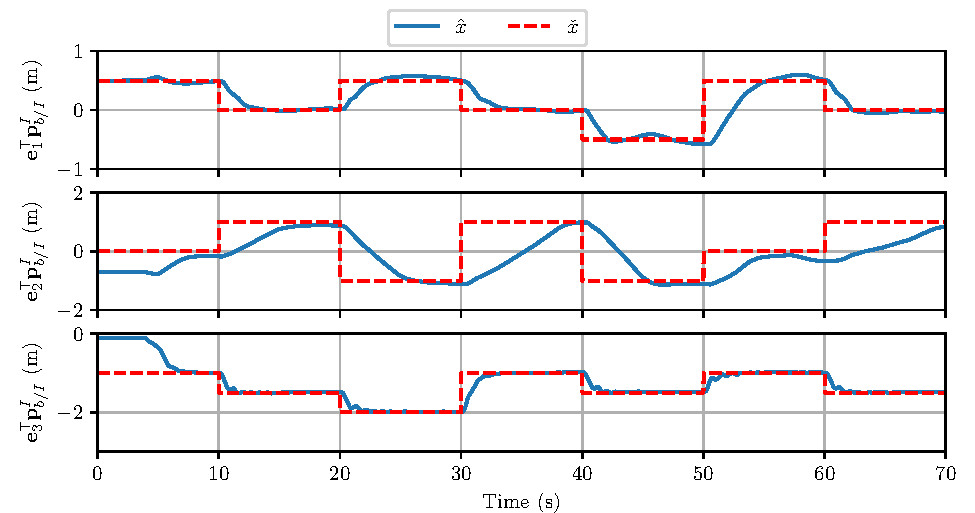
\includegraphics[width=0.4\textwidth]{figures/mocap_wps_position}
  \caption[LQR Hardware Results Flying Waypoints]{Hardware results for the position of the multirotor UAV given step
  inputs to position. The red dotted line is the desired position and the blue
solid line is the estimated position.}
  \label{f:hardware_wps}
\end{figure}

\begin{figure}
  \centering
  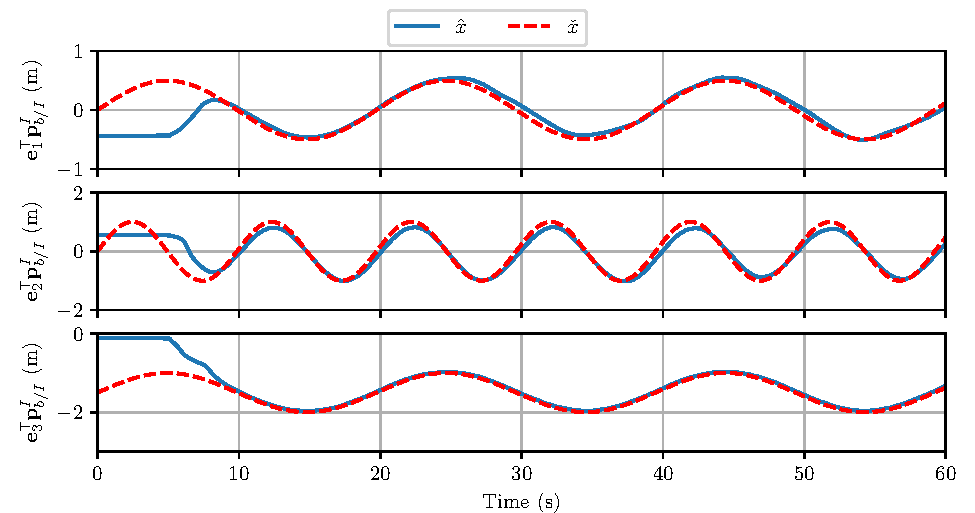
\includegraphics[width=0.4\textwidth]{figures/mocap_fig8_position}
  \caption[LQR Hardware Results Flying a Trajectory]{Hardware results of a multirotor UAV tracking a figure eight
  trajectory. The red dotted line is the desired position and the blue solid
line is the estimated position.}
  \label{f:hardware_fig8}
\end{figure}

\begin{figure}
  \centering
  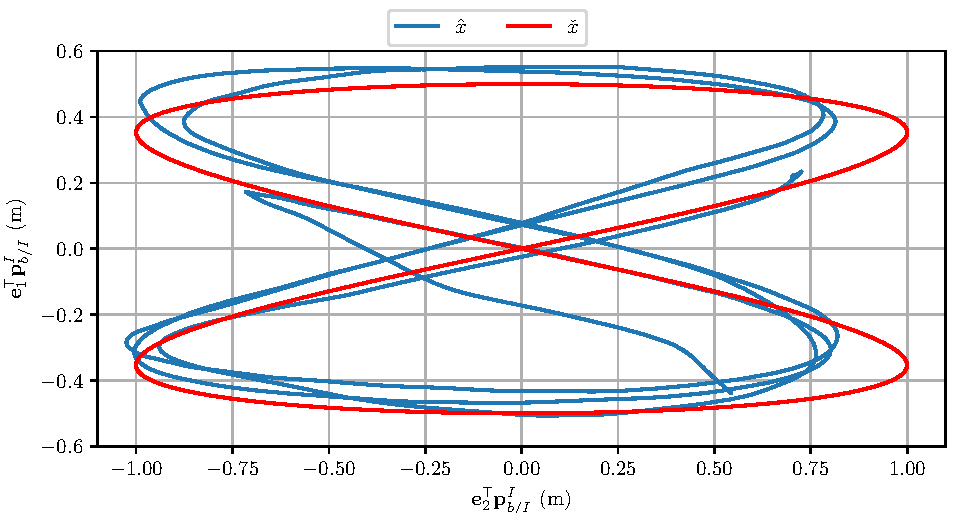
\includegraphics[width=0.4\textwidth]{figures/mocap_fig8_position_2d}
  \caption[Top Down View of LQR Hardware Trajectory]{Top down view of a multirotor UAV tracking a figure eight
  trajectory in hardware. The major deviation in position indicates the time
during take-off when the multirotor must get to the trajectory before following
it. The red solid line is the desired position and the blue solid line is the
estimated position.}
  \label{f:hardware_fig8_2d}
\end{figure}

Fig.~\ref{f:hardware_wps} shows the multirotor position along with the commanded
positions for a waypoint path. The clean step response with minimal overshoot is
notable considering we did not hand tune the LQR gains beyond an initial value
derived from Bryson's rule. Fig. \ref{f:hardware_fig8} shows how well the
multirotor is able to follow the figure-eight trajectory, and Fig.
\ref{f:hardware_fig8_2d} depicts the same flight plotted in two dimensions. The
major deviations visible in this plot depict the take-off and landing portions
of the flight.
